% Options for packages loaded elsewhere
\PassOptionsToPackage{unicode}{hyperref}
\PassOptionsToPackage{hyphens}{url}
\PassOptionsToPackage{dvipsnames,svgnames,x11names}{xcolor}
%
\documentclass[
  letterpaper,
  DIV=11,
  numbers=noendperiod]{scrartcl}

\usepackage{amsmath,amssymb}
\usepackage{iftex}
\ifPDFTeX
  \usepackage[T1]{fontenc}
  \usepackage[utf8]{inputenc}
  \usepackage{textcomp} % provide euro and other symbols
\else % if luatex or xetex
  \usepackage{unicode-math}
  \defaultfontfeatures{Scale=MatchLowercase}
  \defaultfontfeatures[\rmfamily]{Ligatures=TeX,Scale=1}
\fi
\usepackage{lmodern}
\ifPDFTeX\else  
    % xetex/luatex font selection
\fi
% Use upquote if available, for straight quotes in verbatim environments
\IfFileExists{upquote.sty}{\usepackage{upquote}}{}
\IfFileExists{microtype.sty}{% use microtype if available
  \usepackage[]{microtype}
  \UseMicrotypeSet[protrusion]{basicmath} % disable protrusion for tt fonts
}{}
\makeatletter
\@ifundefined{KOMAClassName}{% if non-KOMA class
  \IfFileExists{parskip.sty}{%
    \usepackage{parskip}
  }{% else
    \setlength{\parindent}{0pt}
    \setlength{\parskip}{6pt plus 2pt minus 1pt}}
}{% if KOMA class
  \KOMAoptions{parskip=half}}
\makeatother
\usepackage{xcolor}
\setlength{\emergencystretch}{3em} % prevent overfull lines
\setcounter{secnumdepth}{5}
% Make \paragraph and \subparagraph free-standing
\makeatletter
\ifx\paragraph\undefined\else
  \let\oldparagraph\paragraph
  \renewcommand{\paragraph}{
    \@ifstar
      \xxxParagraphStar
      \xxxParagraphNoStar
  }
  \newcommand{\xxxParagraphStar}[1]{\oldparagraph*{#1}\mbox{}}
  \newcommand{\xxxParagraphNoStar}[1]{\oldparagraph{#1}\mbox{}}
\fi
\ifx\subparagraph\undefined\else
  \let\oldsubparagraph\subparagraph
  \renewcommand{\subparagraph}{
    \@ifstar
      \xxxSubParagraphStar
      \xxxSubParagraphNoStar
  }
  \newcommand{\xxxSubParagraphStar}[1]{\oldsubparagraph*{#1}\mbox{}}
  \newcommand{\xxxSubParagraphNoStar}[1]{\oldsubparagraph{#1}\mbox{}}
\fi
\makeatother

\usepackage{color}
\usepackage{fancyvrb}
\newcommand{\VerbBar}{|}
\newcommand{\VERB}{\Verb[commandchars=\\\{\}]}
\DefineVerbatimEnvironment{Highlighting}{Verbatim}{commandchars=\\\{\}}
% Add ',fontsize=\small' for more characters per line
\usepackage{framed}
\definecolor{shadecolor}{RGB}{241,243,245}
\newenvironment{Shaded}{\begin{snugshade}}{\end{snugshade}}
\newcommand{\AlertTok}[1]{\textcolor[rgb]{0.68,0.00,0.00}{#1}}
\newcommand{\AnnotationTok}[1]{\textcolor[rgb]{0.37,0.37,0.37}{#1}}
\newcommand{\AttributeTok}[1]{\textcolor[rgb]{0.40,0.45,0.13}{#1}}
\newcommand{\BaseNTok}[1]{\textcolor[rgb]{0.68,0.00,0.00}{#1}}
\newcommand{\BuiltInTok}[1]{\textcolor[rgb]{0.00,0.23,0.31}{#1}}
\newcommand{\CharTok}[1]{\textcolor[rgb]{0.13,0.47,0.30}{#1}}
\newcommand{\CommentTok}[1]{\textcolor[rgb]{0.37,0.37,0.37}{#1}}
\newcommand{\CommentVarTok}[1]{\textcolor[rgb]{0.37,0.37,0.37}{\textit{#1}}}
\newcommand{\ConstantTok}[1]{\textcolor[rgb]{0.56,0.35,0.01}{#1}}
\newcommand{\ControlFlowTok}[1]{\textcolor[rgb]{0.00,0.23,0.31}{\textbf{#1}}}
\newcommand{\DataTypeTok}[1]{\textcolor[rgb]{0.68,0.00,0.00}{#1}}
\newcommand{\DecValTok}[1]{\textcolor[rgb]{0.68,0.00,0.00}{#1}}
\newcommand{\DocumentationTok}[1]{\textcolor[rgb]{0.37,0.37,0.37}{\textit{#1}}}
\newcommand{\ErrorTok}[1]{\textcolor[rgb]{0.68,0.00,0.00}{#1}}
\newcommand{\ExtensionTok}[1]{\textcolor[rgb]{0.00,0.23,0.31}{#1}}
\newcommand{\FloatTok}[1]{\textcolor[rgb]{0.68,0.00,0.00}{#1}}
\newcommand{\FunctionTok}[1]{\textcolor[rgb]{0.28,0.35,0.67}{#1}}
\newcommand{\ImportTok}[1]{\textcolor[rgb]{0.00,0.46,0.62}{#1}}
\newcommand{\InformationTok}[1]{\textcolor[rgb]{0.37,0.37,0.37}{#1}}
\newcommand{\KeywordTok}[1]{\textcolor[rgb]{0.00,0.23,0.31}{\textbf{#1}}}
\newcommand{\NormalTok}[1]{\textcolor[rgb]{0.00,0.23,0.31}{#1}}
\newcommand{\OperatorTok}[1]{\textcolor[rgb]{0.37,0.37,0.37}{#1}}
\newcommand{\OtherTok}[1]{\textcolor[rgb]{0.00,0.23,0.31}{#1}}
\newcommand{\PreprocessorTok}[1]{\textcolor[rgb]{0.68,0.00,0.00}{#1}}
\newcommand{\RegionMarkerTok}[1]{\textcolor[rgb]{0.00,0.23,0.31}{#1}}
\newcommand{\SpecialCharTok}[1]{\textcolor[rgb]{0.37,0.37,0.37}{#1}}
\newcommand{\SpecialStringTok}[1]{\textcolor[rgb]{0.13,0.47,0.30}{#1}}
\newcommand{\StringTok}[1]{\textcolor[rgb]{0.13,0.47,0.30}{#1}}
\newcommand{\VariableTok}[1]{\textcolor[rgb]{0.07,0.07,0.07}{#1}}
\newcommand{\VerbatimStringTok}[1]{\textcolor[rgb]{0.13,0.47,0.30}{#1}}
\newcommand{\WarningTok}[1]{\textcolor[rgb]{0.37,0.37,0.37}{\textit{#1}}}

\providecommand{\tightlist}{%
  \setlength{\itemsep}{0pt}\setlength{\parskip}{0pt}}\usepackage{longtable,booktabs,array}
\usepackage{calc} % for calculating minipage widths
% Correct order of tables after \paragraph or \subparagraph
\usepackage{etoolbox}
\makeatletter
\patchcmd\longtable{\par}{\if@noskipsec\mbox{}\fi\par}{}{}
\makeatother
% Allow footnotes in longtable head/foot
\IfFileExists{footnotehyper.sty}{\usepackage{footnotehyper}}{\usepackage{footnote}}
\makesavenoteenv{longtable}
\usepackage{graphicx}
\makeatletter
\def\maxwidth{\ifdim\Gin@nat@width>\linewidth\linewidth\else\Gin@nat@width\fi}
\def\maxheight{\ifdim\Gin@nat@height>\textheight\textheight\else\Gin@nat@height\fi}
\makeatother
% Scale images if necessary, so that they will not overflow the page
% margins by default, and it is still possible to overwrite the defaults
% using explicit options in \includegraphics[width, height, ...]{}
\setkeys{Gin}{width=\maxwidth,height=\maxheight,keepaspectratio}
% Set default figure placement to htbp
\makeatletter
\def\fps@figure{htbp}
\makeatother
% definitions for citeproc citations
\NewDocumentCommand\citeproctext{}{}
\NewDocumentCommand\citeproc{mm}{%
  \begingroup\def\citeproctext{#2}\cite{#1}\endgroup}
\makeatletter
 % allow citations to break across lines
 \let\@cite@ofmt\@firstofone
 % avoid brackets around text for \cite:
 \def\@biblabel#1{}
 \def\@cite#1#2{{#1\if@tempswa , #2\fi}}
\makeatother
\newlength{\cslhangindent}
\setlength{\cslhangindent}{1.5em}
\newlength{\csllabelwidth}
\setlength{\csllabelwidth}{3em}
\newenvironment{CSLReferences}[2] % #1 hanging-indent, #2 entry-spacing
 {\begin{list}{}{%
  \setlength{\itemindent}{0pt}
  \setlength{\leftmargin}{0pt}
  \setlength{\parsep}{0pt}
  % turn on hanging indent if param 1 is 1
  \ifodd #1
   \setlength{\leftmargin}{\cslhangindent}
   \setlength{\itemindent}{-1\cslhangindent}
  \fi
  % set entry spacing
  \setlength{\itemsep}{#2\baselineskip}}}
 {\end{list}}
\usepackage{calc}
\newcommand{\CSLBlock}[1]{\hfill\break\parbox[t]{\linewidth}{\strut\ignorespaces#1\strut}}
\newcommand{\CSLLeftMargin}[1]{\parbox[t]{\csllabelwidth}{\strut#1\strut}}
\newcommand{\CSLRightInline}[1]{\parbox[t]{\linewidth - \csllabelwidth}{\strut#1\strut}}
\newcommand{\CSLIndent}[1]{\hspace{\cslhangindent}#1}

\KOMAoption{captions}{tableheading}
\makeatletter
\@ifpackageloaded{caption}{}{\usepackage{caption}}
\AtBeginDocument{%
\ifdefined\contentsname
  \renewcommand*\contentsname{Table of contents}
\else
  \newcommand\contentsname{Table of contents}
\fi
\ifdefined\listfigurename
  \renewcommand*\listfigurename{List of Figures}
\else
  \newcommand\listfigurename{List of Figures}
\fi
\ifdefined\listtablename
  \renewcommand*\listtablename{List of Tables}
\else
  \newcommand\listtablename{List of Tables}
\fi
\ifdefined\figurename
  \renewcommand*\figurename{Figure}
\else
  \newcommand\figurename{Figure}
\fi
\ifdefined\tablename
  \renewcommand*\tablename{Table}
\else
  \newcommand\tablename{Table}
\fi
}
\@ifpackageloaded{float}{}{\usepackage{float}}
\floatstyle{ruled}
\@ifundefined{c@chapter}{\newfloat{codelisting}{h}{lop}}{\newfloat{codelisting}{h}{lop}[chapter]}
\floatname{codelisting}{Listing}
\newcommand*\listoflistings{\listof{codelisting}{List of Listings}}
\makeatother
\makeatletter
\makeatother
\makeatletter
\@ifpackageloaded{caption}{}{\usepackage{caption}}
\@ifpackageloaded{subcaption}{}{\usepackage{subcaption}}
\makeatother

\ifLuaTeX
  \usepackage{selnolig}  % disable illegal ligatures
\fi
\usepackage{bookmark}

\IfFileExists{xurl.sty}{\usepackage{xurl}}{} % add URL line breaks if available
\urlstyle{same} % disable monospaced font for URLs
\hypersetup{
  pdftitle={My title},
  pdfauthor={First author; Another author},
  colorlinks=true,
  linkcolor={blue},
  filecolor={Maroon},
  citecolor={Blue},
  urlcolor={Blue},
  pdfcreator={LaTeX via pandoc}}


\title{My title\thanks{Code and data are available at:
\url{https://github.com/RohanAlexander/starter_folder}.}}
\usepackage{etoolbox}
\makeatletter
\providecommand{\subtitle}[1]{% add subtitle to \maketitle
  \apptocmd{\@title}{\par {\large #1 \par}}{}{}
}
\makeatother
\subtitle{My subtitle if needed}
\author{First author \and Another author}
\date{November 14, 2024}

\begin{document}
\maketitle
\begin{abstract}
First sentence. Second sentence. Third sentence. Fourth sentence.
\end{abstract}


\section{Introduction}\label{introduction}

Overview paragraph

Estimand paragraph

Results paragraph

Why it matters paragraph

Telegraphing paragraph: The remainder of this paper is structured as
follows. Section~\ref{sec-data}\ldots.

\section{Data}\label{sec-data}

\subsection{Overview}\label{overview}

For this study, we utilize data from Project Hammer, a Canadian
initiative designed to monitor grocery prices across major retailers in
Canada. The Project Hammer dataset was collected from eight prominent
Canadian grocery vendors---Voila, T\&T, Loblaws, No Frills, Metro,
Galleria, Walmart, and Save-On-Foods---between February 28, 2024, and
the latest available data load in the database {[}
citeProjectHammerData{]}. This dataset enables us to investigate price
fluctuations, identify pricing trends, and explore potential competitive
or collusive patterns within the Canadian grocery sector. Project Hammer
aims to support regulatory efforts by providing data on price
transparency, making it suitable for academic research and potential
legal analysis. Following data processing and cleaning procedures
outlined in Section 3.2, the dataset was structured to allow an analysis
of historical price changes and vendor-specific price patterns. The
dataset contains 1,996,969 rows and 5 columns, with variables capturing
product (product name), vendor\_name (name of the grocery retailer),
price\_current (current product price at the time of recording),
price\_old (previous recorded price for the product), and
price\_difference (difference between the current and old prices). Price
data is recorded in Canadian dollars and captures a broad range of
grocery items from various categories, including fresh produce, dairy,
pantry staples, and household items. To ensure the quality and
consistency of the data, we focused on removing missing values and
imputing outlier prices when necessary. For this analysis, we excluded
entries with extreme price fluctuations beyond three standard
deviations, as these could represent temporary discounts or data
recording anomalies. This cleaning process provides a balanced and
accurate reflection of grocery pricing, allowing for robust statistical
analysis on vendor-specific trends and average price comparisons across
product types. By narrowing the scope to recent data, Project Hammer's
dataset captures real-time fluctuations in grocery pricing, providing
timely insights into potential market dynamics and consumer price
impacts. The analysis allows for future investigation of temporal price
trends, vendor-based price differences, and, more broadly, consumer
affordability in a market facing rising cost-of-living pressures.

\subsection{Measurement}\label{measurement}

Some paragraphs about how we go from a phenomena in the world to an
entry in the dataset.

\subsection{Outcome variables}\label{outcome-variables}

Add graphs, tables and text. Use sub-sub-headings for each outcome
variable or update the subheading to be singular.

Some of our data is of penguins (Figure~\ref{fig-bills}), from Horst,
Hill, and Gorman (2020).

\begin{figure}

\centering{

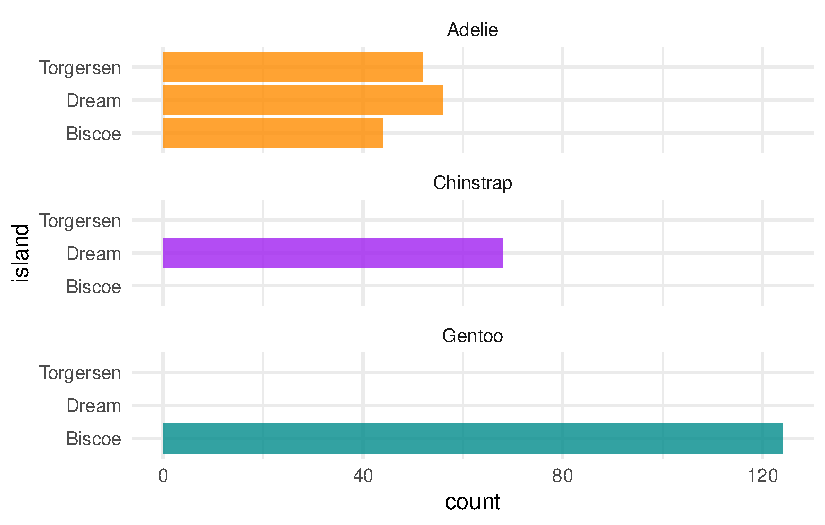
\includegraphics{paper_files/figure-pdf/fig-bills-1.pdf}

}

\caption{\label{fig-bills}Bills of penguins}

\end{figure}%

Talk more about it.

And also planes (Figure~\ref{fig-planes}). (You can change the height
and width, but don't worry about doing that until you have finished
every other aspect of the paper - Quarto will try to make it look nice
and the defaults usually work well once you have enough text.)

\begin{figure}

\centering{

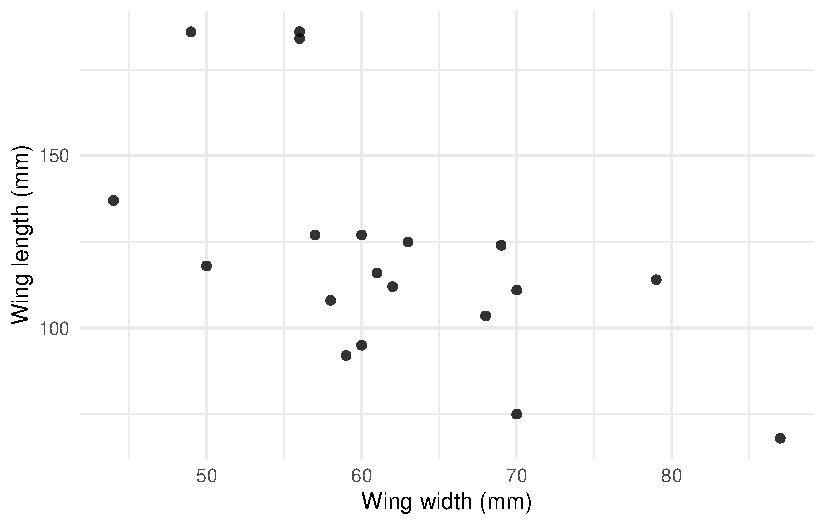
\includegraphics{paper_files/figure-pdf/fig-planes-1.pdf}

}

\caption{\label{fig-planes}Relationship between wing length and width}

\end{figure}%

Talk way more about it.

\subsection{Predictor variables}\label{predictor-variables}

Add graphs, tables and text.

Use sub-sub-headings for each outcome variable and feel free to combine
a few into one if they go together naturally.

\section{Model}\label{model}

Our modeling approach seeks to explore and quantify the relationship
between previous grocery prices, vendor identities, and price
differences in the current prices observed within Canadian grocery
stores. This analysis employs a Bayesian linear regression model
implemented via the \texttt{stan\ \_glm} function in the
\texttt{rstanarm} package to examine how factors such as historical
prices, vendor differences, and observed price changes impact current
prices for various grocery items.

In this model, \texttt{price\_current} serves as the response variable,
while \texttt{price\_old}, \texttt{vendor\_name}, and
\texttt{price\_difference} act as predictor variables. The linear
regression model assumes a Gaussian distribution for the response
variable \texttt{price\_current}, allowing for a straightforward
interpretation of the estimated parameters.

\subsection{Model set-up}\label{model-set-up}

The model includes the following predictor variables:

\begin{itemize}
\item
  Previous Price (\texttt{price\_old}): The price of the product in a
  previous time period.
\item
  Vendor (\texttt{vendor\_name}): A categorical variable representing
  the grocery store chain selling the product, capturing vendor-specific
  pricing differences.
\item
  Price Difference (\texttt{price\_difference}): The difference between
  the current and previous price, which may indicate market or
  vendor-specific pricing adjustments.
\end{itemize}

The model can be represented mathematically as follows:

\begin{align*}
    y_i \mid \mu_i, \sigma &\sim \text{Normal}(\mu_i, \sigma) \\
    \mu_i &= \beta_0 + \beta_1 \cdot \text{Previous Price}_i + \beta_2 \cdot \text{Vendor}_i + \beta_3 \cdot \text{Price Difference}_i \\
    \epsilon_i &\sim \text{Normal}(0, \sigma^2)
\end{align*}

\textbf{Where:}

\begin{itemize}
    \item $\beta_0$ is the intercept term, representing the baseline estimate of $price_{current}$
    \item $\beta_1$, $\beta_2$, and $\beta_3$ are the coefficients representing the effects of $price_{old}$, $vendor_{name}$ and $price_{difference}$ on $price_{current}$.
    \item $\sigma^2$represents the variance of the error term, capturing unexplained variability in current prices.
\end{itemize}

The model is executed in \texttt{R} (R Core Team 2023) using the
\texttt{rstanarm} package (Goodrich et al. 2022), with priors set to
regularize the estimates and prevent overfitting. Specifically, we use a
normal prior for the coefficients, centered at zero with moderate
variance, to ensure stable estimates without overly restrictive
assumptions.

\subsubsection{Model justification}\label{model-justification}

The selection of a linear regression model for this analysis is based on
the continuous nature of \texttt{price\_current}, which allows us to
quantify how previous pricing, vendor, and price changes influence
current pricing. Existing economic theories suggest that previous prices
and historical pricing patterns are often predictive of current pricing,
especially in competitive retail markets where price sensitivity and
vendor-specific strategies play significant roles. The inclusion of
\texttt{price\_old} as a predictor aligns with time-series economic
models where past data points inform future values.

Additionally, vendor differences, represented by \texttt{vendor\_name},
capture potential competitive dynamics in the Canadian grocery market.
Vendors may adopt distinct pricing strategies or respond differently to
market conditions, and the inclusion of this categorical variable
enables an analysis of these patterns across various major grocery
chains. The \texttt{price\_difference} variable, which represents recent
price changes, provides an understanding of market adjustments and
reflects fluctuations potentially influenced by external factors, such
as supply chain constraints or inflation.

The Bayesian approach was selected for its flexibility in incorporating
prior information and its robustness in handling uncertainty within
small or moderate sample sizes. Furthermore, Bayesian methods allow us
to capture the posterior distributions of the parameters, which can be
used to evaluate the strength and credibility of each predictor's effect
on current prices. This approach also aligns with the objectives of
Project Hammer by facilitating a transparent and probabilistically
rigorous analysis of grocery pricing trends.

In summary, this model helps explain the primary factors of current
grocery prices in Canadian stores, accounting for both historical prices
and vendor effects. By utilizing Bayesian framework, this analysis
provides a clear quantification of the influence of each predictor while
allowing for robust estimation and interpretability in the context of
economic and competitive pricing strategies.

\section{Results}\label{results}

The results of our analysis of the Project Hammer dataset explain
important findings about pricing trends across major Canadian grocery
vendors. By examining factors such as prior pricing
(\texttt{price\_old}), vendor identities (\texttt{vendor\_name}), and
recent price changes (\texttt{price\_difference}), we assess how these
variables affect current prices (\texttt{price\_current}). The following
sections summarize key findings, supported by visualizations that
highlight trends and relationships within the data.

\subsection{Vendor-Specific Price
Trends}\label{vendor-specific-price-trends}

We begin by examining average current prices (\texttt{price\_current})
across different grocery vendors to identify potential pricing
variations in the Canadian grocery market.

\begin{Shaded}
\begin{Highlighting}[]
\DocumentationTok{\#\#\#\# Read data \#\#\#\#}
\CommentTok{\# Load the cleaned dataset}
\NormalTok{analysis\_data }\OtherTok{\textless{}{-}} \FunctionTok{read\_csv}\NormalTok{(}\StringTok{"C:/Users/eliza/Downloads/hammer{-}3{-}compressed/cleaned\_price\_changes.csv"}\NormalTok{, }\AttributeTok{show\_col\_types =} \ConstantTok{FALSE}\NormalTok{)}

\CommentTok{\# Generate plot for Average Current Price by Vendor}
\NormalTok{vendor\_price\_plot }\OtherTok{\textless{}{-}}\NormalTok{ analysis\_data }\SpecialCharTok{\%\textgreater{}\%}
  \FunctionTok{group\_by}\NormalTok{(vendor\_name) }\SpecialCharTok{\%\textgreater{}\%}
  \FunctionTok{summarize}\NormalTok{(}\AttributeTok{avg\_price\_current =} \FunctionTok{mean}\NormalTok{(price\_current, }\AttributeTok{na.rm =} \ConstantTok{TRUE}\NormalTok{)) }\SpecialCharTok{\%\textgreater{}\%}
  \FunctionTok{ggplot}\NormalTok{(}\FunctionTok{aes}\NormalTok{(}\AttributeTok{x =} \FunctionTok{reorder}\NormalTok{(vendor\_name, avg\_price\_current), }\AttributeTok{y =}\NormalTok{ avg\_price\_current)) }\SpecialCharTok{+}
  \FunctionTok{geom\_bar}\NormalTok{(}\AttributeTok{stat =} \StringTok{"identity"}\NormalTok{, }\AttributeTok{fill =} \StringTok{"skyblue"}\NormalTok{) }\SpecialCharTok{+}
  \FunctionTok{coord\_flip}\NormalTok{() }\SpecialCharTok{+}
  \FunctionTok{labs}\NormalTok{(}
    \AttributeTok{title =} \StringTok{"Average Current Price by Vendor"}\NormalTok{,}
    \AttributeTok{x =} \StringTok{"Vendor"}\NormalTok{,}
    \AttributeTok{y =} \StringTok{"Average Current Price (CAD)"}
\NormalTok{  ) }\SpecialCharTok{+}
  \FunctionTok{theme\_minimal}\NormalTok{()}

\CommentTok{\# Display the plot}
\NormalTok{vendor\_price\_plot}
\end{Highlighting}
\end{Shaded}

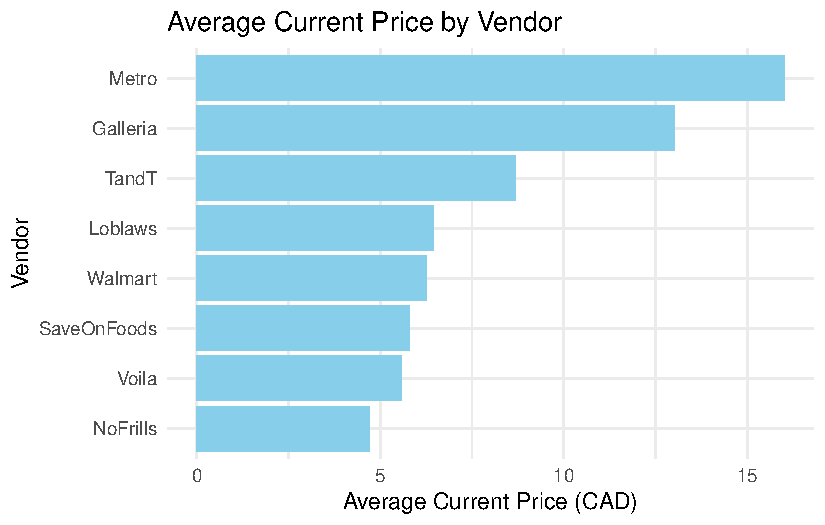
\includegraphics{paper_files/figure-pdf/unnamed-chunk-4-1.pdf}

Figure 1: Average Current Price by Vendor. This bar plot shows the
average price of products sold by each grocery vendor in Canadian
dollars (CAD). Variations in pricing suggest differences in market
positioning or pricing strategies among vendors, with some retailers
consistently offering higher or lower prices across product categories.

\subsection{Price Difference Analysis}\label{price-difference-analysis}

We further analyze \texttt{price\_difference}, which captures the change
between the current price (\texttt{price\_current}) and the previous
price (\texttt{price\_old}). This variable provides insights into recent
price adjustments across vendors.

\begin{Shaded}
\begin{Highlighting}[]
\CommentTok{\# Average price difference by vendor}
\NormalTok{price\_diff\_plot }\OtherTok{\textless{}{-}}\NormalTok{ analysis\_data }\SpecialCharTok{\%\textgreater{}\%}
  \FunctionTok{group\_by}\NormalTok{(vendor\_name) }\SpecialCharTok{\%\textgreater{}\%}
  \FunctionTok{summarize}\NormalTok{(}\AttributeTok{avg\_price\_difference =} \FunctionTok{mean}\NormalTok{(price\_difference, }\AttributeTok{na.rm =} \ConstantTok{TRUE}\NormalTok{)) }\SpecialCharTok{\%\textgreater{}\%}
  \FunctionTok{ggplot}\NormalTok{(}\FunctionTok{aes}\NormalTok{(}\AttributeTok{x =} \FunctionTok{reorder}\NormalTok{(vendor\_name, avg\_price\_difference), }\AttributeTok{y =}\NormalTok{ avg\_price\_difference)) }\SpecialCharTok{+}
  \FunctionTok{geom\_bar}\NormalTok{(}\AttributeTok{stat =} \StringTok{"identity"}\NormalTok{, }\AttributeTok{fill =} \StringTok{"coral"}\NormalTok{) }\SpecialCharTok{+}
  \FunctionTok{coord\_flip}\NormalTok{() }\SpecialCharTok{+}
  \FunctionTok{labs}\NormalTok{(}
    \AttributeTok{title =} \StringTok{"Average Price Difference by Vendor"}\NormalTok{,}
    \AttributeTok{x =} \StringTok{"Vendor"}\NormalTok{,}
    \AttributeTok{y =} \StringTok{"Average Price Difference (CAD)"}
\NormalTok{  ) }\SpecialCharTok{+}
  \FunctionTok{theme\_minimal}\NormalTok{()}
\NormalTok{price\_diff\_plot}
\end{Highlighting}
\end{Shaded}

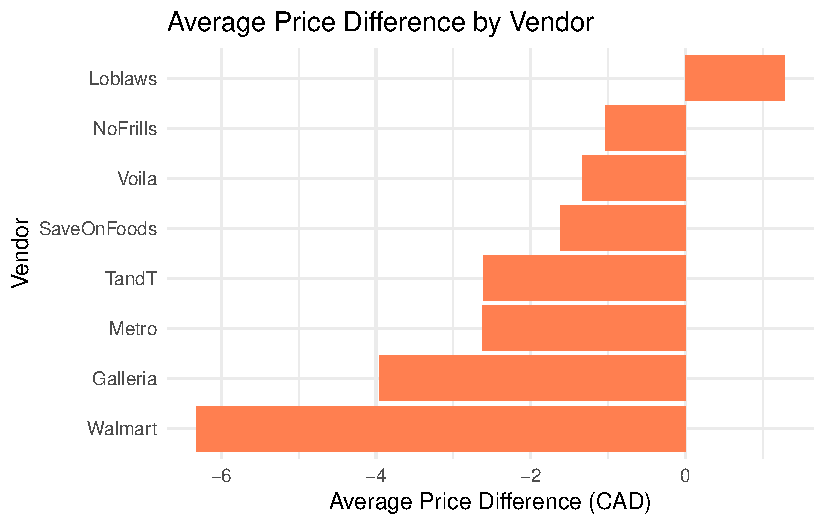
\includegraphics{paper_files/figure-pdf/unnamed-chunk-5-1.pdf}

Figure 2: Average Price Difference by Vendor. This bar plot shows the
average price change per vendor, highlighting retailers with the most
significant pricing adjustments. Positive differences suggest recent
price increases, while negative differences indicate reductions,
reflecting possible discounting or competitive pricing strategies.

\subsection{Relationship Between Previous and Current
Prices}\label{relationship-between-previous-and-current-prices}

We assess the relationship between previous prices (\texttt{price\_old})
and current prices (\texttt{price\_current}) to understand price
consistency and potential price elasticity across products.

\begin{Shaded}
\begin{Highlighting}[]
\CommentTok{\# Scatter plot of previous price vs. current price}
\NormalTok{price\_relationship\_plot }\OtherTok{\textless{}{-}} \FunctionTok{ggplot}\NormalTok{(analysis\_data, }\FunctionTok{aes}\NormalTok{(}\AttributeTok{x =}\NormalTok{ price\_old, }\AttributeTok{y =}\NormalTok{ price\_current)) }\SpecialCharTok{+}
  \FunctionTok{geom\_point}\NormalTok{(}\AttributeTok{alpha =} \FloatTok{0.4}\NormalTok{, }\AttributeTok{color =} \StringTok{"blue"}\NormalTok{) }\SpecialCharTok{+}
  \FunctionTok{geom\_smooth}\NormalTok{(}\AttributeTok{method =} \StringTok{"lm"}\NormalTok{, }\AttributeTok{color =} \StringTok{"red"}\NormalTok{) }\SpecialCharTok{+}
  \FunctionTok{labs}\NormalTok{(}
    \AttributeTok{title =} \StringTok{"Relationship Between Previous and Current Prices"}\NormalTok{,}
    \AttributeTok{x =} \StringTok{"Previous Price (CAD)"}\NormalTok{,}
    \AttributeTok{y =} \StringTok{"Current Price (CAD)"}
\NormalTok{  ) }\SpecialCharTok{+}
  \FunctionTok{theme\_minimal}\NormalTok{()}
\NormalTok{price\_relationship\_plot}
\end{Highlighting}
\end{Shaded}

\begin{verbatim}
`geom_smooth()` using formula = 'y ~ x'
\end{verbatim}

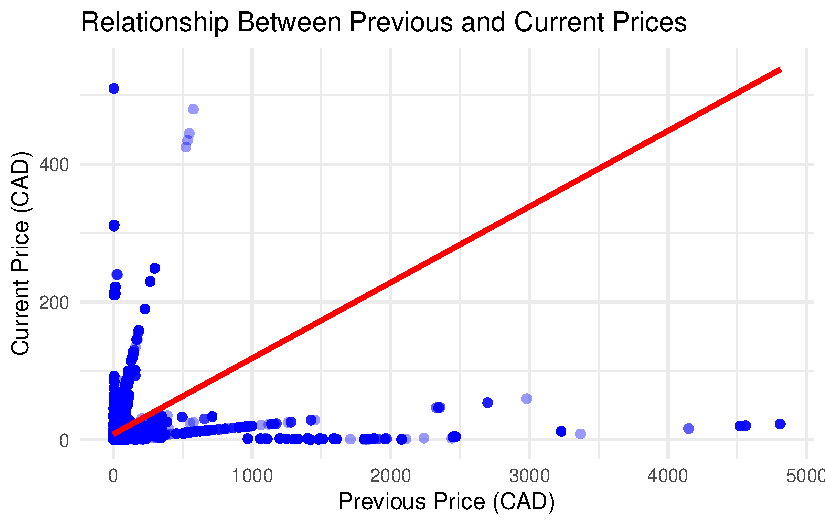
\includegraphics{paper_files/figure-pdf/unnamed-chunk-6-1.pdf}

Figure 3: Relationship Between Previous and Current Prices. This scatter
plot with a linear regression line shows the correlation between
previous and current prices. A positive relationship would indicate that
higher previous prices predict higher current prices, implying potential
price stability or gradual price changes in the grocery market.

\subsection{Distribution of Price
Differences}\label{distribution-of-price-differences}

To further explore pricing dynamics, we examine the distribution of
\texttt{price\_difference}, capturing both price increases and decreases
across the dataset.

\begin{Shaded}
\begin{Highlighting}[]
\CommentTok{\# Calculate mean and standard deviation of price\_difference}
\NormalTok{mean\_diff }\OtherTok{\textless{}{-}} \FunctionTok{mean}\NormalTok{(analysis\_data}\SpecialCharTok{$}\NormalTok{price\_difference, }\AttributeTok{na.rm =} \ConstantTok{TRUE}\NormalTok{)}
\NormalTok{sd\_diff }\OtherTok{\textless{}{-}} \FunctionTok{sd}\NormalTok{(analysis\_data}\SpecialCharTok{$}\NormalTok{price\_difference, }\AttributeTok{na.rm =} \ConstantTok{TRUE}\NormalTok{)}

\CommentTok{\# Filter out extreme values beyond 3 standard deviations}
\NormalTok{filtered\_data }\OtherTok{\textless{}{-}}\NormalTok{ analysis\_data }\SpecialCharTok{\%\textgreater{}\%}
  \FunctionTok{filter}\NormalTok{(price\_difference }\SpecialCharTok{\textgreater{}=}\NormalTok{ (mean\_diff }\SpecialCharTok{{-}} \DecValTok{3} \SpecialCharTok{*}\NormalTok{ sd\_diff),}
\NormalTok{         price\_difference }\SpecialCharTok{\textless{}=}\NormalTok{ (mean\_diff }\SpecialCharTok{+} \DecValTok{3} \SpecialCharTok{*}\NormalTok{ sd\_diff))}

\CommentTok{\# Plot histogram with filtered data}
\NormalTok{price\_difference\_hist }\OtherTok{\textless{}{-}} \FunctionTok{ggplot}\NormalTok{(filtered\_data, }\FunctionTok{aes}\NormalTok{(}\AttributeTok{x =}\NormalTok{ price\_difference)) }\SpecialCharTok{+}
  \FunctionTok{geom\_histogram}\NormalTok{(}\AttributeTok{bins =} \DecValTok{30}\NormalTok{, }\AttributeTok{fill =} \StringTok{"lightgreen"}\NormalTok{, }\AttributeTok{color =} \StringTok{"black"}\NormalTok{) }\SpecialCharTok{+}
  \FunctionTok{labs}\NormalTok{(}
    \AttributeTok{title =} \StringTok{"Distribution of Price Differences (Filtered)"}\NormalTok{,}
    \AttributeTok{x =} \StringTok{"Price Difference (CAD)"}\NormalTok{,}
    \AttributeTok{y =} \StringTok{"Frequency"}
\NormalTok{  ) }\SpecialCharTok{+}
  \FunctionTok{theme\_minimal}\NormalTok{()}
\NormalTok{price\_difference\_hist}
\end{Highlighting}
\end{Shaded}

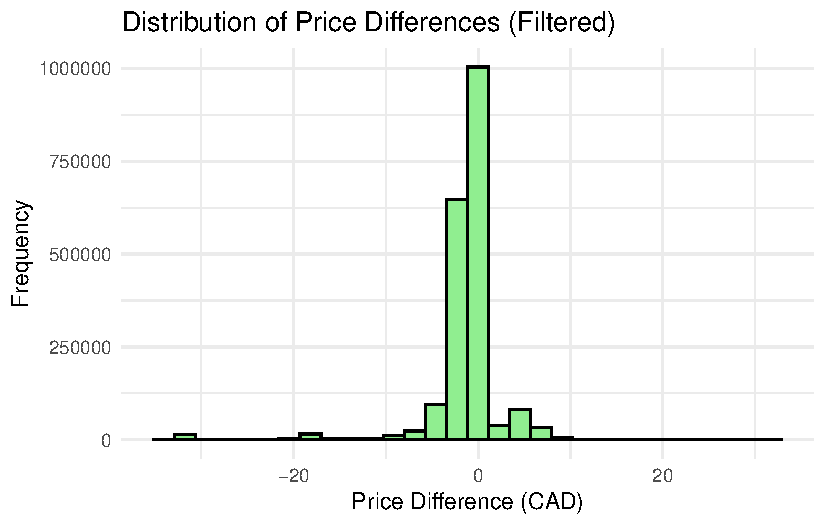
\includegraphics{paper_files/figure-pdf/unnamed-chunk-7-1.pdf}

Figure 4: Distribution of Price Differences (Filtered). This histogram
illustrates the frequency of price changes across products, with extreme
values beyond three standard deviations removed for clarity. The
concentration around zero suggests that small price adjustments are most
common, while the presence of both negative and positive values
indicates instances of both price increases and decreases. This
distribution provides insight into the stability and variability of
pricing across vendors.

\section{Discussion}\label{discussion}

\subsection{Interpretation of Grocery Pricing
Dynamics}\label{interpretation-of-grocery-pricing-dynamics}

This study investigates the primary factors influencing current grocery
prices in Canada by examining the Project Hammer dataset. Our Bayesian
regression model reveals that prior prices (\texttt{price\_old}), vendor
identity (\texttt{vendor\_name}), and recent price differences
(\texttt{price\_difference}) play significant roles in determining
current prices. The influence of previous prices indicates price
continuity across time, suggesting that grocery items tend to exhibit
relatively stable pricing patterns with minor adjustments.
Vendor-specific effects highlight the role of retailer pricing
strategies, with some vendors maintaining consistently higher or lower
prices. These vendor variations may reflect differences in market
positioning, operational costs, or competitive strategies, impacting
price consistency across the grocery sector.

Additionally, the presence of both positive and negative values in the
\texttt{price\_difference} variable illustrates the prevalence of both
price increases and decreases, underscoring the dynamic nature of
grocery pricing in response to external market forces. External factors,
such as supply chain disruptions, inflation, and seasonal demand
fluctuations, likely contribute to the observed variability. This model
highlights the complexity of pricing dynamics and the importance of
historical pricing and vendor-specific factors in shaping current
grocery prices across major Canadian retailers.

\subsection{Implications for Competition and Consumer
Costs}\label{implications-for-competition-and-consumer-costs}

The findings from Project Hammer have broader implications for both
competition in the grocery sector and consumer expenses. Vendor-specific
price differences suggest that some retailers adopt competitive pricing
strategies to attract cost-sensitive consumers, while others may
leverage brand loyalty or perceived quality to justify higher prices. In
this context, price-sensitive consumers may benefit from exploring
pricing variations across vendors to find the best deals, while
retailers may face pressure to adjust their prices to remain
competitive.

The stability of historical prices as a predictor of current prices also
highlights potential concerns about price rigidity in certain product
categories. This rigidity may limit the effectiveness of competition, as
vendors might rely on historical price baselines rather than actively
adjusting prices in response to market demand. Policymakers interested
in promoting competition in the grocery sector could consider
encouraging more frequent pricing updates or transparency in pricing
strategies, particularly for staple items that heavily impact household
budgets.

\subsection{Limitations of Data and
Model}\label{limitations-of-data-and-model}

This analysis has several limitations that may impact the accuracy and
comprehensiveness of our findings. First, the dataset is limited to
major grocery chains, which may not capture price variations across
smaller or regional stores that could offer different pricing
structures. Additionally, the lack of granular product-level data limits
our ability to analyze category-specific trends (e.g., dairy versus
produce) or regional differences within the same vendor.

The model's focus on historical prices, vendor identity, and price
differences also excludes potential external factors that may influence
pricing, such as seasonal demand, promotions, or supply chain
constraints. Including additional variables, such as the frequency of
price adjustments or regional economic indicators, could enhance the
model's predictive power and provide a more comprehensive view of
grocery pricing dynamics.

\subsection{Future Research Direction}\label{future-research-direction}

Future research could build on this work by incorporating a wider range
of variables, including product-specific attributes, seasonal factors,
and promotional data, to capture a broader spectrum of influences on
grocery prices. Exploring how demographic factors, such as income levels
in different regions, correlate with price patterns across vendors could
offer insights into the socio-economic impacts of grocery pricing on
different communities.

Increasing the model's granularity to analyze price dynamics at the
regional or product-category level would provide a deeper understanding
of how specific items are priced within the same store or across
regions. Additionally, expanding the analysis to include other sectors,
such as online grocery prices or specialty stores, could provide a more
holistic view of the Canadian grocery market.

Incorporating machine learning techniques could also improve the model's
adaptability to rapidly changing market conditions, allowing for more
nuanced forecasts of pricing trends. This approach could be particularly
useful in the face of ongoing challenges such as inflation and supply
chain disruptions, offering a valuable tool for policymakers and
consumers interested in understanding and mitigating grocery costs in
Canada.

\newpage

\appendix

\section*{Appendix}\label{appendix}
\addcontentsline{toc}{section}{Appendix}

\section{Additional data details}\label{additional-data-details}

\section{Model details}\label{sec-model-details}

\subsection{Posterior predictive
check}\label{posterior-predictive-check}

\newpage

\section*{References}\label{references}
\addcontentsline{toc}{section}{References}

\phantomsection\label{refs}
\begin{CSLReferences}{1}{0}
\bibitem[\citeproctext]{ref-rstanarm}
Goodrich, Ben, Jonah Gabry, Imad Ali, and Sam Brilleman. 2022.
{``{rstanarm: {Bayesian} applied regression modeling via {Stan}}.''}
\url{https://mc-stan.org/rstanarm/}.

\bibitem[\citeproctext]{ref-palmerpenguins}
Horst, Allison Marie, Alison Presmanes Hill, and Kristen B Gorman. 2020.
\emph{{palmerpenguins: Palmer Archipelago (Antarctica) penguin data}}.
\url{https://doi.org/10.5281/zenodo.3960218}.

\bibitem[\citeproctext]{ref-citeR}
R Core Team. 2023. \emph{{R: A Language and Environment for Statistical
Computing}}. Vienna, Austria: R Foundation for Statistical Computing.
\url{https://www.R-project.org/}.

\end{CSLReferences}




\end{document}
